\documentclass{article}
\usepackage{graphicx} % Required for inserting images
\usepackage{tabularx}
\usepackage{amssymb}
\usepackage{amsmath}
\usepackage{amsthm}
\usepackage{listings}
\usepackage[swedish]{babel}
\usepackage{hyperref} 
\usepackage{mathtools}
\usepackage{color}
\usepackage{titlesec}
\usepackage{sectsty}
\usepackage[a4paper, margin=2cm]{geometry}
\usepackage{booktabs}
\usepackage{caption}
\usepackage{subcaption}
\usepackage{float}
\usepackage{tikz}


\renewcommand{\thesection}{\arabic{section}.}
\renewcommand{\thesubsection}{\alph{subsection})}
\subsectionfont{\normalfont\bfseries\fontsize{10}{12}\selectfont}

\newcommand{\independent}{\perp\!\!\!\!\perp}

\title{SF1930 Projekt}
\author{Vilhelm Karlin}
\date{\today}

\begin{document}
\maketitle

\section{Uppvärmning}
\subsection{Alla betyg i dataramen är för närvarande tal mellan 0 och 10. 
Normalisera dessa värden i dataramen så att de är mellan 0 och 1.}

För att normalisera datan så itererade jag helt enkelt över de relevanta kolumnerna och dividerade varje värde med 10. 

\subsection{Gör ett histogram för alla trickbetyg för trick 1-4. Vad observerar du? 
Finns det ett visst värde som dyker upp oftare än de andra? Om så är fallet, hur står detta värde i jämförelse med de andra?}

Som syns i figur Fig\ref{fig:1b} så är det enskilt vanligaste värdet 0. Resterande värden är ungefär grupperande mellan 0.7 och 0.9.
Inga värden finns mellan 0.1 och 0.4.

\subsection{For varje trick 1-4 skapa en ny kolumn med namnet 'make i' för i = 1, 2, 3, 4 så att värdet av 'make i' i en given rad är 1 om skateboardåkaren landade trick i och 0 annars.}
Detta implementeras enkelt genom att introducera fyra nya kolumner, en för varje trick. Dessa fylls sedan med 1 om skateboardåkaren landade trick i och 0 annars.

\subsection{För varje skateboardåkare skatta sannolikheten att ett trick får ett betyg som är större än 0.6 givet att 
skateboardåkaren landar tricket. Vad är sannolikheten att skateboardåkaren inte lyckas landa ett visst trick? Vad observerar du? 
Relatera dina observationer till era observationer i del (b).}

Som syns i Tab\ref{tab:1d} så är det endast två skateboardåkare som inte fick betyg större än 0.6 på något av sina gjorda trick.
Detta rimmar väl med observationerna i Fig\ref{fig:1b} där värdena antingen var 0 eller större än runt 0.6.

\subsection{Gör ett spridningsdiagram för runbetyg 1 mot runbetyg 2. Ser du någon tydligt korrelation från diagrammet?} \label{sec:1e}

Korrelationen mellan runbetyg 1 och runbetyg 2 är väldigt svag och ingen tydlig trend kan urskiljas i Fig\ref{fig:1e}.
Korrelationskoefficienten $\rho = 0.19$. Jag anser därmed att det är rimligt att anta att runbetyg 1 och runbetyg 2 är oberoende.

\clearpage  % Start a new page for figures and tables

\begin{figure}[htbp]
    \centering
    
    \begin{minipage}{0.45\textwidth}
        \centering
        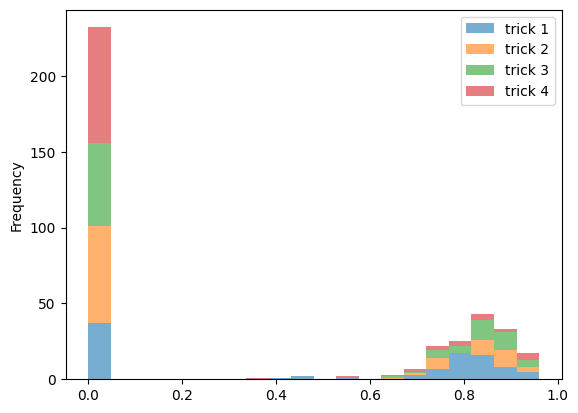
\includegraphics[width=\textwidth]{Figures/1b.png}
        \caption{Histogram för trickbetyg 1-4.}
        \label{fig:1b}
    \end{minipage}
    \hfill
    \begin{minipage}{0.45\textwidth}
        \centering
        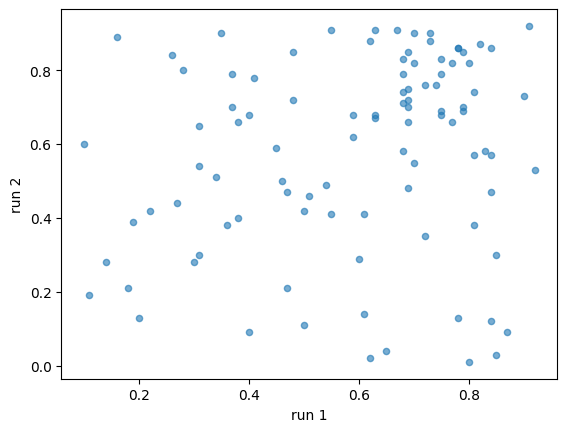
\includegraphics[width=\textwidth]{Figures/1e.png}
        \caption{Caption for figure 2.}
        \label{fig:1e}
    \end{minipage}
    
\end{figure}

\begin{table}[htbp]
    \centering
    \begin{tabular}{lrr}
      \toprule
      \textbf{ID} & \textbf{Gjorda trick} & \textbf{Andel med betyg större än 0.6} \\
      \midrule
      Berger     &      2 &              1.00 \\
      Decenzo    &      7 &              1.00 \\
      Eaton      &      5 &              1.00 \\
      Foy        &      6 &              1.00 \\
      Fynn       &      6 &              1.00 \\
      Gustavo    &      8 &              1.00 \\
      Hoban      &      8 &              1.00 \\
      Hoefler    &      7 &              1.00 \\
      Horigome   &      9 &              1.00 \\
      Huston     &      3 &              1.00 \\
      Jordan     &      8 &              1.00 \\
      Joslin     &      9 &              1.00 \\
      Majerus    &      3 &              0.33 \\
      McClung    &      1 &              0.00 \\
      Midler     &      4 &              1.00 \\
      Milou      &      9 &              1.00 \\
      Mota       &      3 &              1.00 \\
      Oliveira   &      5 &              1.00 \\
      O’neill    &      3 &              1.00 \\
      Papa       &      7 &              1.00 \\
      Pudwill    &      3 &              0.33 \\
      Ribeiro C  &      3 &              1.00 \\
      \bottomrule
    \end{tabular}
    \caption{Betyg större än 0.6 givet att skateboardåkaren landar tricket}
    \label{tab:1d}
\end{table}
\newpage

\section{En frekventistisk modell.}
\subsection{Ge en punktskattning för varje $\theta_i$, sannolikheten att skateboardåkaren i landar ett trick.}
Via momentmetoden kan vi enklet visa att $\hat{\theta_i} = \frac{1}{n}\sum_{j=1}^n v_{ij}$ är en punktskattning för $\theta_i$ om vi antar att $V_i \sim \text{Ber}(\theta_i)$.
Eftersom $V_i \independent Z_i$ så kan vi helt enkelt tillämpa detta på värdena i 'make i' kolumnerna och får därmed punktskattningarna för $\theta_i$ som visas i Tab\ref{tab:freq_params}. 
\\ \\
Notera att vi endast kommer betrakta skateboardåkare som tävlar i LCQ:n från och med nu.

% Ge en punktskattning för parametrarna [αi,βi]T för varje skateboardåkare i. Finns det skateboardåkare för vilka din valda punktskattning inte existera? I så fall föreslå en alternativ punktskattning för dessa αi, βi. Motivera dina val punktskattningar.
\subsection{Ge en punkskattning för parametrarna $[\alpha_i, \beta_i]^T$ för varje skateboardåkare $i$. 
Finns det skateboardåkare för vilka din valda punktskattning inte existera? 
I så fall föreslå en alternativ punktskattning för dessa $\alpha_i, \beta_i$. Motivera dina val punktskattningar.}

Vi använder momentmetoden för att skatta $\alpha_i$ och $\beta_i$ med hjälp av utfall från $Z_i \sim \text{Beta}(\alpha_i, \beta_i)$.

\begin{equation*}
    E[Z_i] = \frac{\alpha_i}{\alpha_i + \beta_i}, Var[Z_i] = \frac{\alpha_i\beta_i}{(\alpha_i + \beta_i)^2(\alpha_i + \beta_i + 1)} \\
\end{equation*}
Vi vill behöver alltså lösa följande system för $\alpha, \beta$ för att få momentmetodens skattningar.
\begin{equation*}
    \bar{z_i} = \frac{\alpha_i}{\alpha_i + \beta_i}, s_i^2 = \frac{\alpha_i\beta_i}{(\alpha_i + \beta_i)^2(\alpha_i + \beta_i + 1)} \\
\end{equation*}
Där $\bar{z_i}$ och $s_i^2$ är stickprovsmedelvärdet och stickprovsvariansen för $Z_i$. Genom att lösa ut $\alpha_i$ och $\beta_i$ ur ekvationerna ovan får vi följande skattningar.

\begin{align}
    \hat{\alpha_i} &= \bar{z_i} (\frac{\bar{z_i}(1-\bar{z_i})}{s_i^2} - 1) \\
    \hat{\beta_i} &= (1-\bar{z_i}) (\frac{\bar{z_i}(1-\bar{z_i})}{s_i^2} - 1)
\end{align}
Skattningarna existerar för alla skateboardåkare förutom Santiago som endast har ett godkänt trick. Han får skattningen $\hat{\alpha}_{\text{Santiago}} = 10 \bar{z}_{\text{Santiago}}, \hat{\beta}_{\text{Santiago}} = 10(1-\bar{z}_{\text{Santiago}})$.
Denna är väntevärdesriktig och ganska konservativ då han har i särklass lägst $E[Z_i]$ av alla skateboardåkare. Samtidigt kommer det ej vara relevant då $\hat{\theta}_{\text{Santiago}} = 0.08$ är så låg att han ej kommer kunna kvalificera sig till finalen.
Punkskattningarna kan ses i Tab\ref{tab:freq_params}.

\subsection{Föreslå en modell för $Y_i$ och ge en punktskattning för dina modells parametrar. Motivera dina val för modell och punktskattning.}
Utifrån observationen från del 1\ref{sec:1e} så antar vi att $Y_{i1}, Y_{i2}$ är oberoende och likafördelade.
Vi kan därmed även modellera runs med en betafördelning, nämligen $Y_i \sim \text{Beta}(a_i, b_i)$. 
Vi tillämpar momentmetoden för att skatta $a_i, b_i$, precis som ovan och resultatet kan ses i Tab\ref{tab:freq_params}.

\subsection{Använd din modell för $[X_i,Y_i]^T$ för att simulera 5000 LCQ:ar och för varje simulering extrahera de fyra skateboardåkare $\vec{W} = [W_1,W_2,W_3,W_4]^T$ med
de högsta totalbetygen. Vad är typvärdet för $\vec{W}_1, ..., \vec{W}_{5000}$? De riktiga vinnarna för LCQ:en är Gustavo, Hoban, Eaton, Decenzo.
Hur många av de riktiga vinnarna förutsägs av typvärdet? Vad är skattade sannolikheten för de riktiga vinnarna baserat på dina simuleringar? Av typvärdet?}

För att simulera en skateboardåkares totala poäng under ett LCQ så kan vi helt enkelt använda våra punkskattningar för att
simulera 4 $X_i$ och 2 $Y_i$, sedan kan vi summera den största $Y_i$ och de två största $X_i$ för att få totalpoängen för den tävlingen.
Vi kör sedan 5000 sådana simuleringar för varje skateboardåkare och därmed får vi våra 5000 $\mathbf{W}_j$.
\\ \\
Typvärdet är Eaton, Hoban, Jordan, Shirai. Denna sker i 1.08\% av fallen. Sannolikheten för de riktiga vinnarna är 0.04\%. 
Om vi betraktar utfallen individuellt får vi att de vanligaste top 4 medlemmarna är Eaton (49\%), Jordan (48\%), Shirai (46\%) och Hoban (43\%). 
Gustavo och Decenzo har sannolikheterna 31\% och 33\% att vara top 4.

\begin{table}[t]
    \centering
    \caption{Frequentistiska punktskattningar för skateboardåkarna.}
    \label{tab:freq_params}
    \begin{tabular}{lrrrrr}
        \toprule
        i & $\hat{\theta}$ & $\hat{\alpha}$ & $\hat{\beta}$ & $\hat{a}$ & $\hat{b}$ \\
        \midrule
        Decenzo   & 0.44 & 24.46 & 5.11 & 4.16 & 2.83 \\
        Eaton     & 0.62 & 75.41 & 20.05 & 103.57 & 36.87 \\
        Foy       & 0.50 & 51.59 & 9.10 & 3.51 & 4.09 \\
        Gustavo   & 0.40 & 70.64 & 17.52 & 1.23 & 0.86 \\
        Hoban     & 0.40 & 107.70 & 15.03 & 3.63 & 2.10 \\
        Hoefler   & 0.44 & 32.52 & 9.40 & 1.75 & 0.97 \\
        Jordan    & 0.40 & 23.06 & 3.64 & 3.61 & 1.23 \\
        Majerus   & 0.38 & 2.91 & 2.72 & 1.76 & 2.47 \\
        Midler    & 0.33 & 43.72 & 10.42 & 1.29 & 0.82 \\
        Mota      & 0.25 & 24.01 & 6.77 & 4.06 & 4.57 \\
        Oliveira  & 0.42 & 68.88 & 17.87 & 5.39 & 4.04 \\
        O'neill   & 0.25 & 1252.67 & 232.71 & 0.60 & 0.73 \\
        Papa      & 0.44 & 22.31 & 6.35 & 2.16 & 2.07 \\
        Ribeiro C & 0.25 & 194.78 & 56.01 & 1.80 & 1.52 \\
        Santiago  & 0.08 & 4.70 & 5.30 & 2.68 & 4.34 \\
        Shirai    & 0.40 & 20.58 & 2.35 & 1.84 & 1.10 \\
        \bottomrule
    \end{tabular}
\end{table}

\newpage
\section{En bayesiansk modell.}

\subsection{Föreslå en simultan apriorifördelning för parametrarna $[\theta_i, \alpha_i, \beta_i]^T$ för $X_i$ där vi antar $\theta_i \independent \alpha_i, \beta_i$ för alla $i$. Motivera ditt val.}

$\Theta_i \independent A_i, B_i \implies f_{\Theta_i, A_i, B_i}(\theta_i, \beta_i, \alpha_i)=f_{\Theta_i}(\theta_i) f_{A_i, B_i}(\alpha_i, \beta_i)$,
och vi kan därmed behandla $\Theta_i$ och $A_i, B_i$ separat. 

$V_i | \Theta_i = \theta_i \sim Ber(\theta_i)$ har som konjugerad apriorifördelning $Beta(c_i, d_i)$, och vi kommer därmed använda den.
$Z_i | A_i = \alpha_i, B_i = \beta_i \sim Beta(\alpha_i, \beta_i)$ har ingen konjugerad apriorifördelning och är därmed ganska knepig.
Exempel 10.8 från föreläsningarna erbjuder ett bra förslag för en apriorifördelning för $\alpha_i, \beta_i$.
Den bygger på en omparameterisering till dess väntevärde och precisionsmått, $\mu_i = \frac{\alpha_i}{\alpha_i + \beta_i}, \kappa_i = \alpha_i + \beta_i + 1$.
Vi kan då bilda en apriorifördelning, $f_{\mu_i, \kappa_i}(\mu_i, \kappa_i) = f_{\kappa_i | \mu_i}(\kappa_i | \mu_i) f_{\mu_i}(\mu_i)$, där $\kappa_i | \mu_i \sim Gamma(\phi_i, \lambda_i)$ och $\mu_i \sim U(0,1)$.
Detta ger oss fördelningen:
\[
    f_{A_i, B_i}(\alpha_i, \beta_i) = \frac{\lambda^{\phi_i}}{\Gamma(\phi_i)} (\alpha_i + \beta_i + 1)^{\phi_i - 1} e^{-\lambda_i(\alpha_i + \beta_i + 1)} (\alpha_i + \beta_i)^{-1}  
\]
Sammansatt får vi följande funktion för den simultana apriorifördelningen:
\[ 
    f_{\Theta_i, A_i, B_i}(\theta_i, \alpha_i, \beta_i) = 
    (\frac{\Gamma(c_i + d_i)}{\Gamma(c_i) \Gamma(d_i)} \theta_i^{c_i-1} (1-\theta_i)^{d_i-1}) 
    (\frac{\lambda^{\phi_i}}{\Gamma(\phi_i)} (\alpha_i + \beta_i + 1)^{\phi_i - 1} e^{-\lambda_i(\alpha_i + \beta_i + 1)} (\alpha_i + \beta_i)^{-1}) 
\]

\subsection{Generera 5000 slumpmässiga utfall från aposteriorifördelningarna $f_{\Theta_i, A_i, B_i | X_i}(\theta_i, \alpha_i, \beta_i | x_i)$.
Plotta dina resulterande utfall för de marginella aposteriorifördelningarna: \\
$f_{\Theta_i | X_i}(\theta_i | x_i)$ och $f_{A_i, B_i | X_i}(\alpha_i, \beta_i | x_i)$. \\
Beräkna det aposteriori stickprovsmedelvärdet och den aposteriori stickprovvariansen för varje parameter $\theta_i, \alpha_i, \beta_i$ för alla skateboardåkare.}

Jag använder mig av Metropolisalgoritmen för att generera 5000 slumpmässiga utfall från aposteriorifördelningarna.
Metropolisalgoritmen har dessutom har den trevliga egenskapen att jag inte behöver kunna normalisera fördelningen.
Jag använder därmed följande:
\begin{align*}
    f_{\Theta_i, A_i, B_i | \mathbf{X}}(\theta_i, \alpha_i, \beta_i | \mathbf{x}) &\propto f_{\mathbf{X} | \Theta_i, A_i, B_i}(\mathbf{x} | \theta_i, \alpha_i, \beta_i) f_{\Theta_i, A_i, B_i}(\theta_i, \alpha_i, \beta_i) \\
    &\propto \theta_i^{c_i-1} (1-\theta_i)^{d_i-1} (\alpha_i + \beta_i + 1)^{\phi_i - 1} e^{-\lambda_i(\alpha_i + \beta_i + 1)} (\alpha_i + \beta_i)^{-1} \prod\limits_{j=1}^4 f_{X_j | \Theta_i, A_i, B_i}(x_j | \theta_i, \alpha_i, \beta_i)
\end{align*}
Till Metropolisalgoritmen använde jag en standardiserad normalfördelning med standardavvikelse, $\sigma = 0.5$ som hoppfördelning,
4 kedjor, 6000 iterationer per kedja (1000 burn-in iterationer) där jag använde punktskattningarna från ovan som startvärden.
För att få olika startvärden för varje kedja så adderade jag till varje startvärde med $e^q$, där $q$ kommer från en Cauchyfördelning med skalfaktor 0.05.
\\\\
Efter lite experementation fann jag parametrar till apriorifördelningen som gav rimliga resultat. 
Jag använde $c_i=d_i=1$, som val för en icke-informativ fördelning för $\Theta_i$. För $A_i, B_i$, använde jag $\lambda_i=0.5, \phi_i=5$.
Resultaten från min simulering, efter burn-in, kan ses i Fig\ref{fig:3b} och Tab\ref{tab:bayes_params}.

% Föreslå en (simultan) apriorifördelning för parametrarna för din modell Yi från uppgift 2(c) och motivera ditt val. Du får anta att modellens parame- trar för skateboardåkaren i är oberoende av alla andra parametrar inklusive θi,αi och βi. Generera 5000 utfall från aposteriorifördelningen (se till att spara dessa utfall!) och gör ett spridningsdiagram av resultatet. Vad är stick- provsmedelvärdet och stickprovsvariansen för var och en av dina parametrar baserat på dina utfall?
\subsection{Föreslå en (simultan) apriorifördelning för parametrarna för din modell $Y_i$ från uppgift 2(c) och motivera ditt val.
Du får anta att modellens parametrar för skateboardåkaren $i$ är oberoende av alla andra parametrar inklusive $\theta_i, \alpha_i$ och $\beta_i$. 
Generera 5000 utfall från aposteriorifördelningen (se till att spara dessa utfall!) och gör ett spridningsdiagram av resultatet.
Vad är stickprovsmedelvärdet och stickprovsvariansen för var och en av dina parametrar baserat på dina utfall?}

Likt i den frequentistiska modellen så antar vi att $Y_i | \mathcal{A}_i = a_i, \mathcal{B}_i = b_i \sim Beta(a_i, b_i)$. 
Vi kan då använda samma apriorifördelning för $\mathcal{A}_i, \mathcal{B}_i$ som användes för $A_i, B_i$ för $X_i$. Vi använder samma $\lambda_i, \phi_i$ som för $A_i, B_i$ och vi använder Metropolisalgoritmen med samma kedjor, hoppfördelning och knep för startvärdena som ovan och aposteriorifördelningen:
\begin{align*}
    f_{\mathcal{A}_i, \mathcal{B}_i | \mathbf{Y}}(a_i, b_i | \mathbf{y}) &\propto f_{\mathbf{Y} | \mathcal{A}_i, \mathcal{B}_i}(\mathbf{y} | a_i, b_i) f_{\mathcal{A}_i, \mathcal{B}_i}(a_i, b_i) \\
    &\propto (a_i + b_i + 1)^{\phi_i - 1} e^{-\lambda_i(a_i + b_i + 1)} (a_i + b_i)^{-1} \prod\limits_{j=1}^2 f_{Y_j | \mathcal{A}_i, \mathcal{B}_i}(y_j | a_i, b_i)
\end{align*}
Plottarna för de aposteriora fördelningarna kan ses i Fig\ref{fig:3c} och dess nyckeltal i Tab\ref{tab:bayes_params}.

\subsection{Använd din bayesiansk modell för $[X_i,Y_i]^T$ för att simulera 5000 LCQ:ar genom att ta utfall från de lämpliga de aposteriori prediktiva fördelningarna.
Vad är typvärdet av dina utfall $W_1,...,W_{5000}$? Hur många av de riktiga vinnarna förutsägs? Vad är den skattade sannolikheten för de riktiga vinnarna baserat på dina utfall? Av typvärdet?}

Samma metod som för den frekventistiska modellen användes för att simulera LCQ:ar. 
Den enda skillnaden är att olika värden för parametrarna användes för varje LCQ, där jag slumpade fram 1250 stickprov från varje kedja.
\\\\
Typvärdet är Eaton, Hoban, Jordan, Shirai. Denna sker i 1.5\% av fallen. Sannolikheten för de riktiga vinnarna är 0.052\%. 
Om vi betraktar utfallen individuellt får vi att de vanligaste top 4 medlemmarna är Eaton (55\%), Jordan (45\%), Shirai (42\%) och Hoban (42\%). 
Gustavo och Decenzo har sannolikheterna 30\% och 35\% att vara top 4.

\begin{table}[H]
    \centering
    \caption{Aposteriori stickprovsmedelvärdet och den aposteriori stickprovsorvariansen för $\theta_i, \alpha_i, \beta_i$}
    \label{tab:bayes_params}
    \begin{tabular}{l|rr|rr|rr|rr|rr}
        \toprule
        i & $\bar{\theta}$ & $s_{\theta}^2$ & $\bar{\alpha}$ & $s_{\alpha}^2$ & $\bar{\beta}$ & $s_{\beta}^2$ & $\bar{a}$ & $s_{a}^2$ & $\bar{b}$ & $s_{b}^2$ \\
        \midrule
        Decenzo & 0.41 & 0.01 & 14.03 & 19.73 & 3.05 & 1.03 & 6.02 & 3.77 & 3.96 & 1.68 \\
        Eaton & 0.55 & 0.02 & 14.06 & 22.63 & 3.97 & 2.04 & 12.79 & 19.26 & 4.81 & 3.15 \\
        Foy & 0.46 & 0.02 & 15.56 & 24.17 & 2.97 & 1.04 & 4.29 & 2.35 & 5.42 & 3.56 \\
        Gustavo & 0.38 & 0.01 & 16.15 & 24.38 & 4.24 & 1.72 & 2.56 & 0.74 & 1.84 & 0.36 \\
        Hoban & 0.38 & 0.01 & 18.08 & 32.30 & 2.83 & 0.84 & 5.41 & 2.94 & 3.00 & 0.89 \\
        Hoefler & 0.42 & 0.01 & 13.78 & 19.61 & 4.14 & 1.94 & 2.56 & 0.84 & 1.73 & 0.39 \\
        Jordan & 0.38 & 0.01 & 15.91 & 24.94 & 2.70 & 0.77 & 6.74 & 4.45 & 2.29 & 0.51 \\
        Majerus & 0.34 & 0.02 & 5.76 & 5.20 & 5.24 & 4.24 & 3.28 & 1.83 & 5.17 & 4.17 \\
        Midler & 0.31 & 0.02 & 13.33 & 23.08 & 3.37 & 1.83 & 1.60 & 0.45 & 1.51 & 0.41 \\
        Mota & 0.22 & 0.01 & 11.61 & 18.87 & 3.38 & 2.09 & 5.54 & 3.45 & 6.05 & 4.18 \\
        Oliveira & 0.38 & 0.02 & 14.10 & 24.66 & 3.93 & 2.21 & 6.86 & 5.46 & 4.95 & 2.96 \\
        O’neill & 0.24 & 0.01 & 14.20 & 27.12 & 2.95 & 1.69 & 1.73 & 0.47 & 2.25 & 0.77 \\
        Papa & 0.40 & 0.01 & 13.04 & 17.59 & 3.80 & 1.59 & 3.74 & 1.64 & 3.67 & 1.51 \\
        Ribeiro C & 0.24 & 0.01 & 12.94 & 20.33 & 3.96 & 2.59 & 3.69 & 1.88 & 3.28 & 1.47 \\
        Santiago & 0.07 & 0.00 & 6.86 & 10.75 & 7.73 & 12.53 & 3.93 & 1.89 & 6.64 & 5.13 \\
        Shirai & 0.38 & 0.01 & 15.63 & 23.94 & 1.93 & 0.40 & 2.57 & 0.74 & 1.68 & 0.30 \\
        \bottomrule
    \end{tabular}
\end{table}

\begin{figure}[htbp]
    \centering
    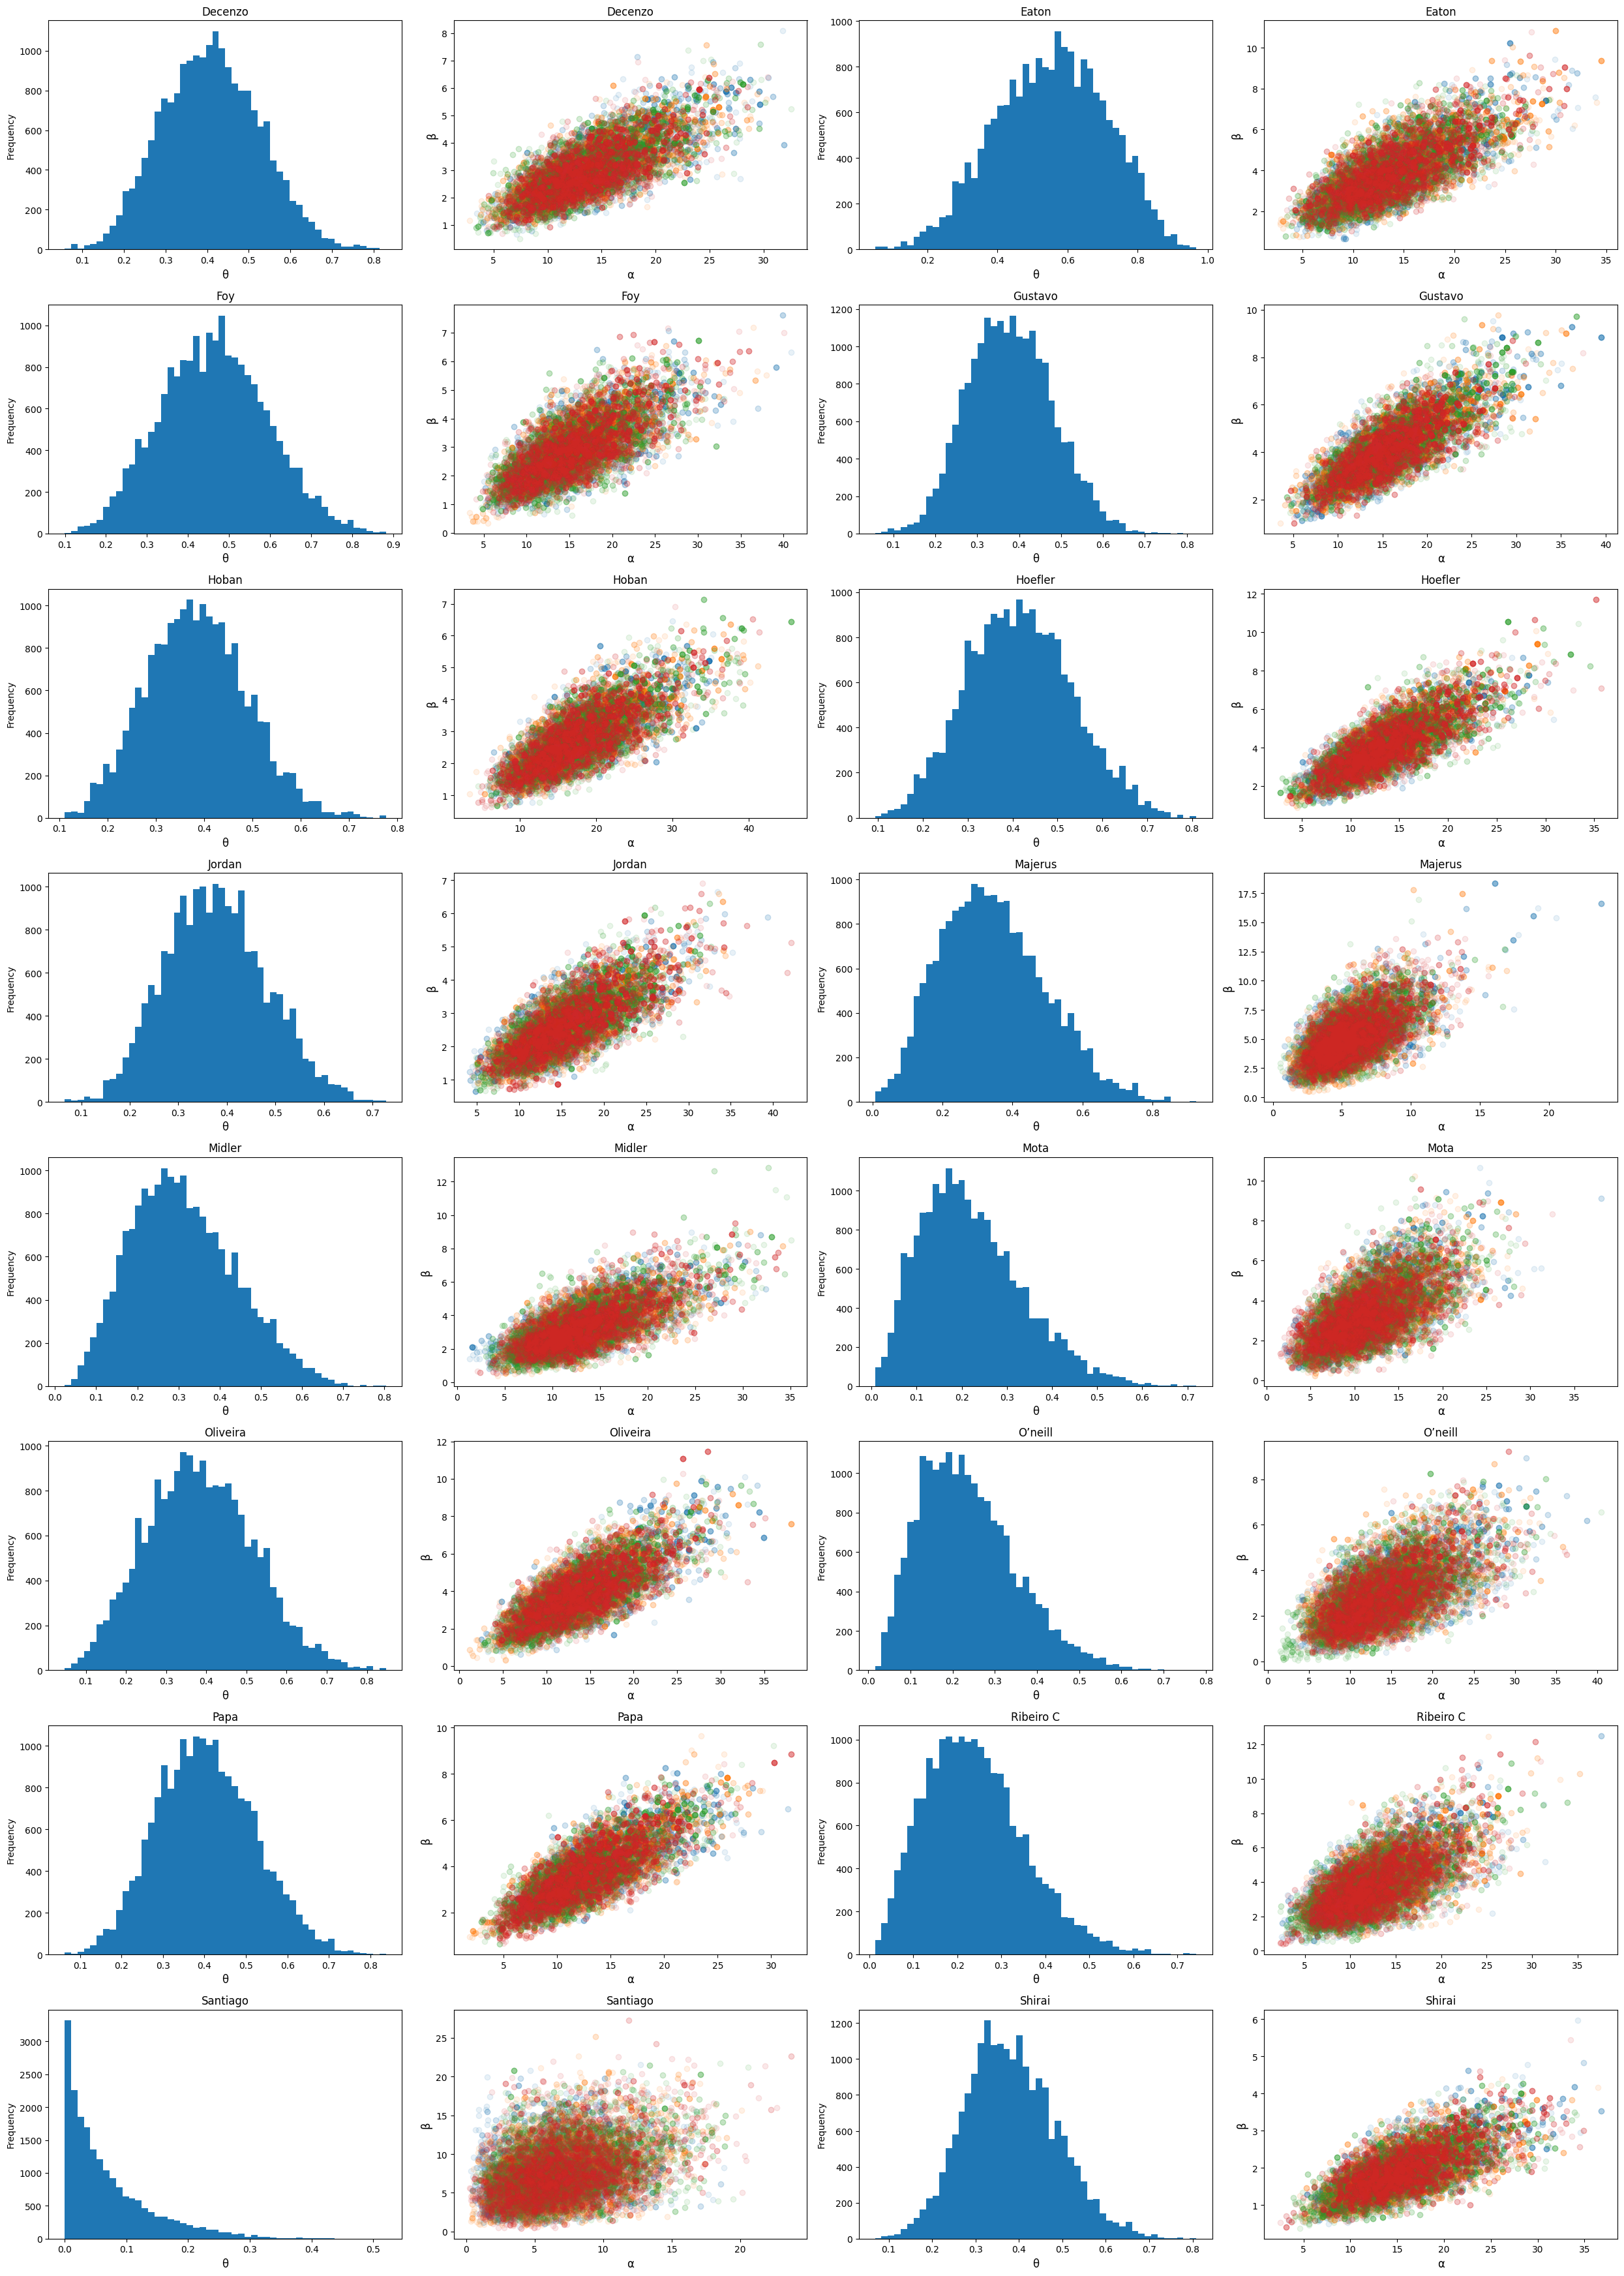
\includegraphics[width=1\textwidth]{Figures/3b.png}
    \caption{Aposterori fördelningar för $\theta_i, \alpha_i, \beta_i$}
    \label{fig:3b}
\end{figure}


\begin{figure}[t]
    \centering
    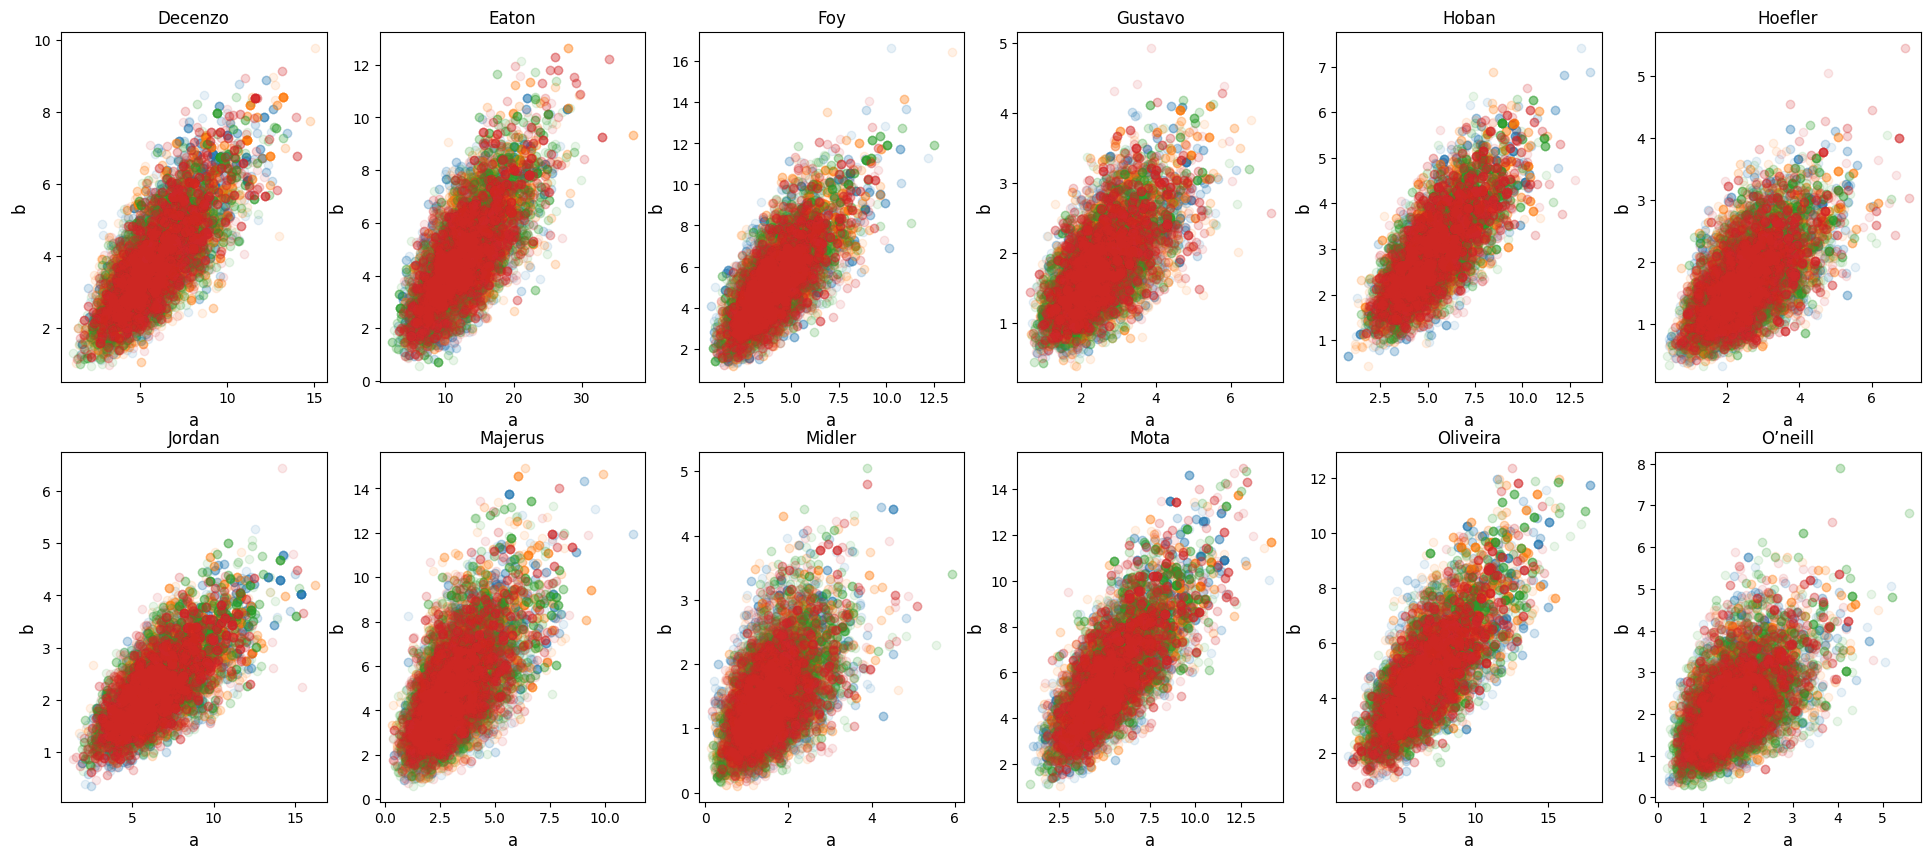
\includegraphics[width=1\textwidth]{Figures/3c.png}
    \caption{Aposterori fördelningar för $a_i, b_i$}
    \label{fig:3c}
\end{figure}

\subsection{I modellen i uppgift 3(d) antog vi att parametrarna $Y_i$ för $Y_i$ och parametrarna $\Theta_i = [\Theta_i, A_i, B_i]^T$ för $X_i$ är oberoende givet data (varför?).
Samtidigt antog vi inte att $\Theta_i \independent A_i, B_i$ är oberoende givet data.
Låt $X_i^{(1)}, X_i^{(2)}, X_i^{(3)}, X_i^{(4)}$ betecknar skateboardåkare $i$:s fyra trickbetyg, låt $Y_i^{(1)}, Y_i^{(2)}$ betecknar skateboardåkare $i$:s två runbetyg och låt $O_i$ betecknar deras totalbetyg.
Rita en acyklisk riktad graf med så få kanter som möjligt så att den simultana fördelningen för $O_i, X_i^{(1)}, X_i^{(2)}, X_i^{(3)}, X_i^{(4)}, Y_i^{(1)}, Y_i^{(2)}, \Theta_i, A_i, B_i$ och $Y_i$ är markovsk med avseende på den.
med avseende på den. Baserat på din graf kan du dra slutsatsen att den marginella aposteriorifördelningen för $\Theta_i, A_i, B_i$ faktoriserar som 
\\$f_{\Theta_i, A_i, B_i | X_i}(\theta_i, \alpha_i, \beta_i | x_i) = f_{\Theta_i | X_i}(\theta_i | x_i)f_{A_i, B_i | X_i}(\alpha_i, \beta_i | x_i)$?
Betrakta dina parametrarna $\Theta_i$ för $Y_i$ och parametrarna $\Theta_i$ för $X_i$. \\Enligt din graf är vårt antagande att $\Theta_i \independent \Theta_i | X_i^{(1)}, X_i^{(2)}, X_i^{(3)}, X_i^{(4)}, Y_i^{(1)}, Y_i^{(2)}$ vettigt?
Kan vi anta oberoenderelationen $\Theta_i \independent \Theta_i | O_i$ om bara datan $o_i$ är givet istället?}

\begin{figure}[h]
    \centering
    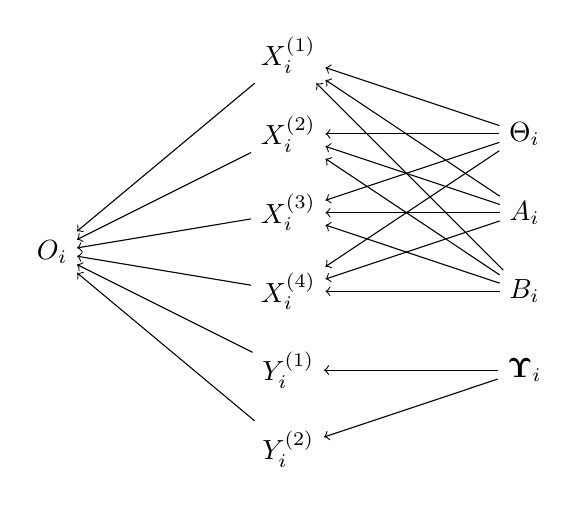
\begin{tikzpicture}
        \centering
        % Nodes
        \node (theta) at (6, 4) {$\Theta_i$};
        \node (a) at (6, 3) {$A_i$};
        \node (b) at (6, 2) {$B_i$};
        \node (upsilon) at (6, 1) {$\mathbf{\Upsilon}_i$};
        \node (x1) at (3, 5) {$X_i^{(1)}$};
        \node (x2) at (3, 4) {$X_i^{(2)}$};
        \node (x3) at (3, 3) {$X_i^{(3)}$};
        \node (x4) at (3, 2) {$X_i^{(4)}$};
        \node (y1) at (3, 1) {$Y_i^{(1)}$};
        \node (y2) at (3, 0) {$Y_i^{(2)}$};
        \node (o) at (0, 2.5) {$O_i$};
        % Edges
        \draw[->] (theta) -- (x1);
        \draw[->] (theta) -- (x2);
        \draw[->] (theta) -- (x3);
        \draw[->] (theta) -- (x4);
        \draw[->] (a) -- (x1);
        \draw[->] (a) -- (x2);
        \draw[->] (a) -- (x3);
        \draw[->] (a) -- (x4);
        \draw[->] (b) -- (x1);
        \draw[->] (b) -- (x2);
        \draw[->] (b) -- (x3);
        \draw[->] (b) -- (x4);
        \draw[->] (upsilon) -- (y1);
        \draw[->] (upsilon) -- (y2);
        \draw[->] (x1) -- (o);
        \draw[->] (x2) -- (o);
        \draw[->] (x3) -- (o);
        \draw[->] (x4) -- (o);
        \draw[->] (y1) -- (o);
        \draw[->] (y2) -- (o);
    \end{tikzpicture}
    \caption{LCQ graf, $\mathcal{G}$}
    \label{fig:hierarki}
\end{figure}
Vi antog att $\mathbf{\Theta} \independent \mathbf{\Upsilon} | \mathbf{X} = \mathbf{x}$ eftersom trick och runs är olika kategorier i tävlingen och den enas data bör därmed ej påverka den andras fördelning.
Dessutom gör det modellen enklare.
\\\\
Enligt grafen så är det tyligt att $\Theta_i \not\independent A_i, B_i | \mathbf{X}$ då information kan flöda från $\Theta_i$ till $A_i, B_i$ via $\mathbf{X}$ eftersom $\Theta_i, A_i, B_i$ alla är föräldrar till $\mathbf{X}$.
Eftersom våra stokastiska variablar är markovska med avseende på $\mathcal{G}$ så gäller:
\[
    f_{\Theta_i, A_i, B_i | X_i}(\theta_i, \alpha_i, \beta_i | x_i) \neq f_{\Theta_i | X_i}(\theta_i | x_i)f_{A_i, B_i | X_i}(\alpha_i, \beta_i | x_i)
\]
Grafen visar att $\mathbf{\Upsilon} \independent \mathbf{\Theta} | X_i^{(1)}, X_i^{(2)}, X_i^{(3)}, X_i^{(4)}, Y_i^{(1)}, Y_i^{(2)}$, då det inte finns någon stig mellan våra $\mathbf{X}_i$ och $\mathbf{Y}_i$.
Däremot är $\mathbf{\Upsilon} \not\independent \mathbf{\Theta} | O_i$ då båda $\mathbf{\Upsilon}$ och $\mathbf{\Theta}$ är förfädrar till $O_i$.

\newpage
\section{En bayesiansk modell med en hierarki.}


\end{document}